Nim przejdziemy do omówienia modeli obliczeń równoległych zajmiemy się omówieniem modelu RAM. 


Model RAM (\emph{Random Access Machine}) odpowiada rozważaniom zawartym w \ref{subsec:algorytmy_sekwencyjne}. Zakłada on:
\begin{enumerate}
\item{Istnienie pewnego procesora wyposażonego w:
\begin{enumerate}
\item skończoną listę instrukcji, które może on realizować (tabela \ref{tab:ram_instructions}).
\item pewną liczbę rejestrów arytmetycznych procesora \(R_1, R_2, \dots, R_n\), \(n>1\) które mogą przechowywać dowolne skończone liczby w zapisie binarnym.
\item specjalny rejestr sterujący \(L\) zwany licznikiem programu.
\end{enumerate}}
\item Istnienie pamięci złożonej z potencjalnie nieskończonej liczby komórek \(M_i, \, i=1, 2, 3, \dots\) (rys. \ref{fig:neumann}) w których można przechowywać dowolną skończoną liczbę w zapisie binarnym.
\item Stały czas zapisu i odczytu wartości do/z komórki pamięci (inaczej \emph{dostęp swobodny}).

\end{enumerate}


\begin{figure}[h]
\centering
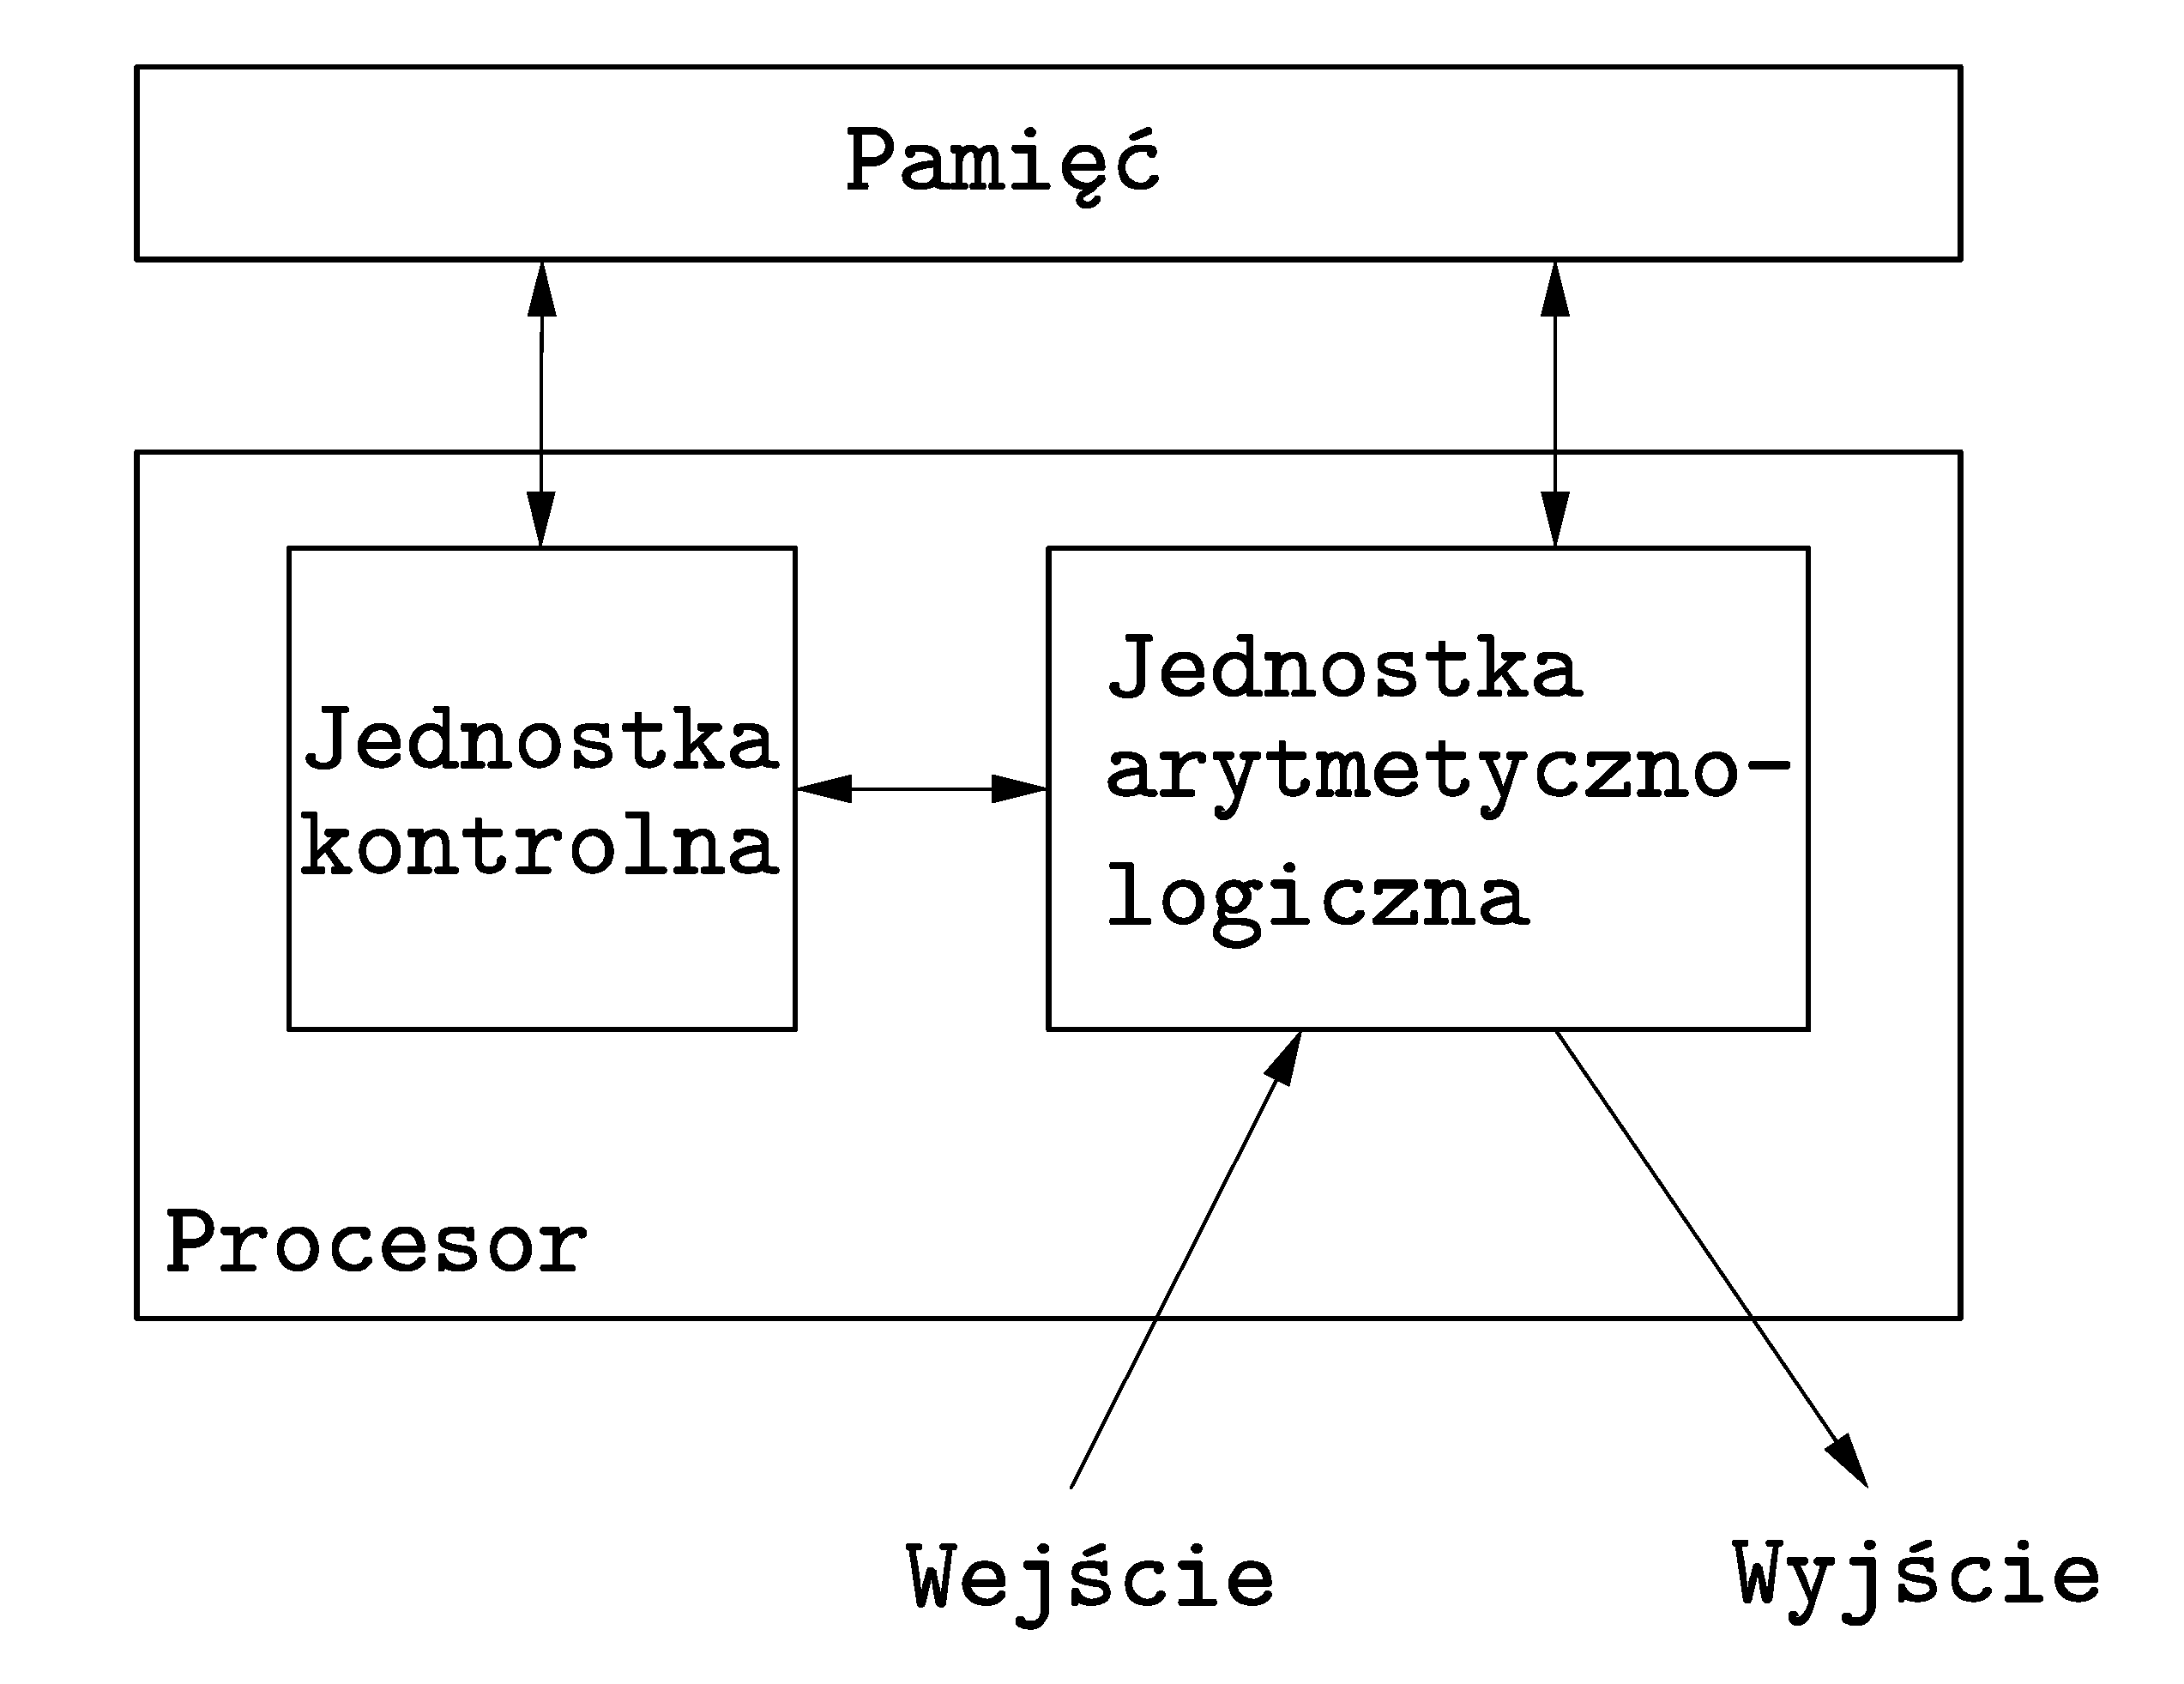
\includegraphics[width=9cm]{images/Rys_Neumann.eps}

\caption{Model obliczeń sekwencyjnych RAM – architektura Von Neumanna}
\label{fig:neumann}
\end{figure}


% \begin{figure}[h]
% \centering
% 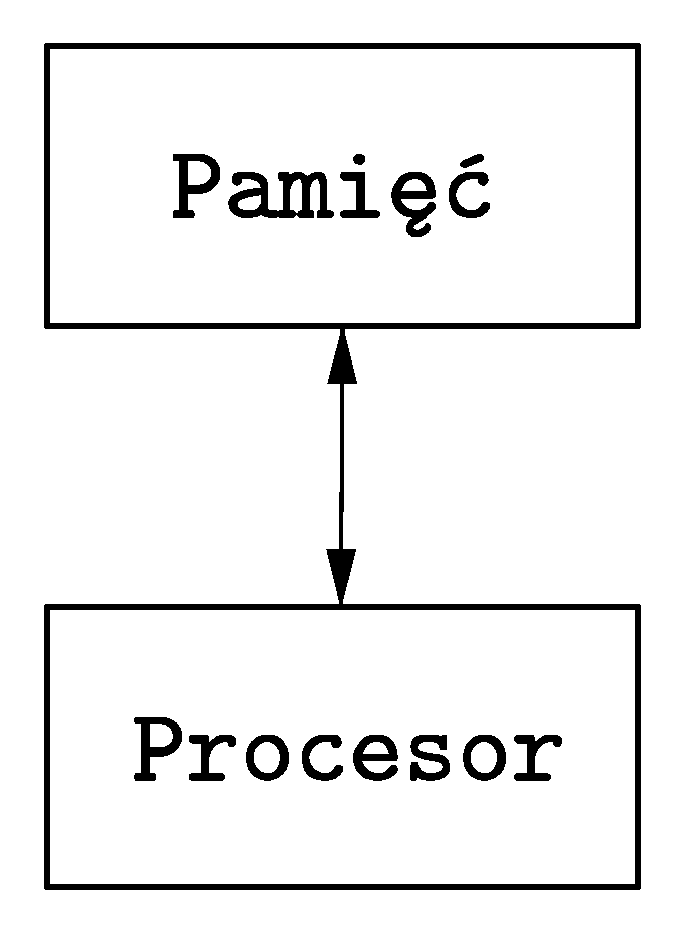
\includegraphics[width=7em]{images/Rys_RAM.eps}
% \caption{Model obliczeń sekwencyjnych RAM}
% \label{fig:ram}
% 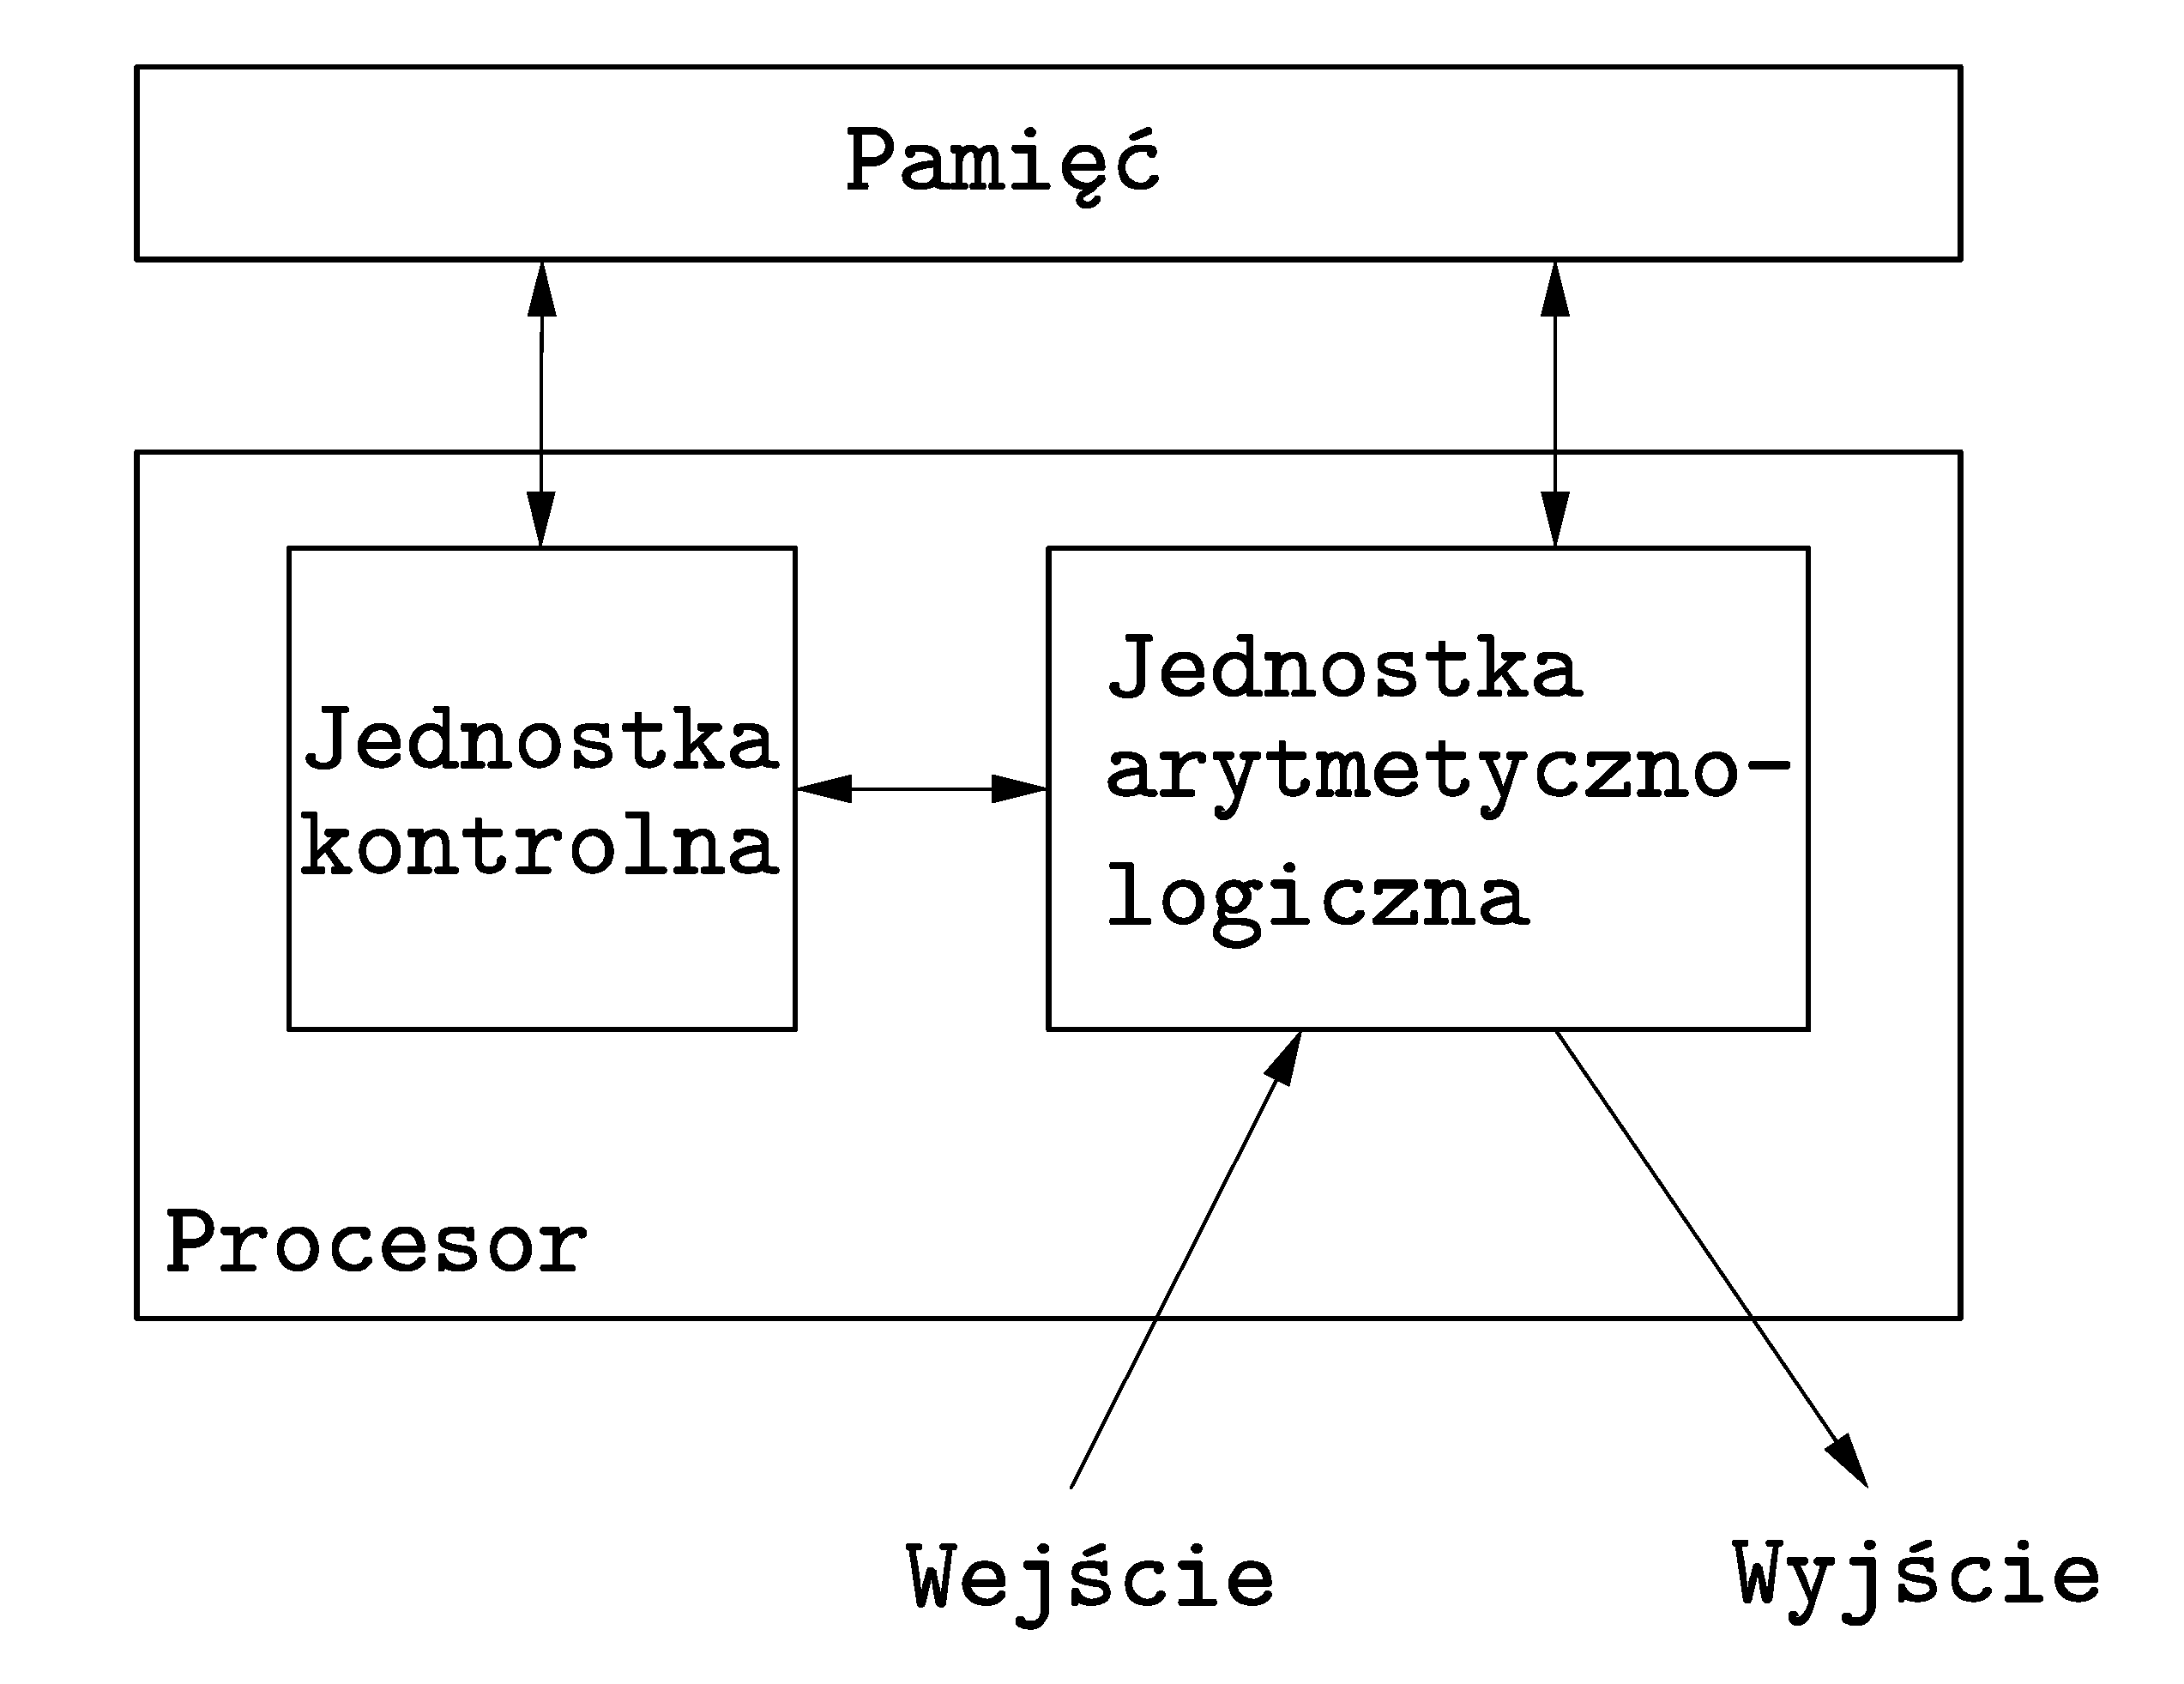
\includegraphics[width=7cm]{images/Rys_Neumann.eps}
% \end{figure}

\begin{table}[H]
\begin{center}
\caption{Przykładowa lista instrukcji procesora\cite{Czech}}
\label{tab:ram_instructions}
\begin{tabular}{|l|c|l|}
\hline
Instrukcja & Argument & Znaczenie \\ \hline
\texttt{LOAD} & \(k, a\) & \(R_k:=w(a)\) \\
\texttt{STORE} & \(k, b\) & \(M_{w(b)}:=R_{k}\) \\
\texttt{ADD} & \(k, c\) & \(R_{k}:=R_{k}+w(c)\) \\
\texttt{SUB} & \(k, c\) & \(R_{k}:=R_{k}-w(c)\)\\
\texttt{MULT} & \(k, c\) & \(R_{k}:=R_{k} \times w(c)\)\\
\texttt{DIV} & \(k, c\) & \(R_{k}:=\lfloor R_{k}/w(c)\rfloor\) \\
\texttt{JUMP} &  \(i\) & \(L:=i\) \\
\texttt{JPOS} & \(k,i\) & \texttt{if} \(R_k>0\) \texttt{then} \(L:=i\) \texttt{else} \(L:=L+1\) \\
\texttt{JZERO} & \(k,i\) & \texttt{if} \(R_k==0\) \texttt{then} \(L:=i\) \texttt{else} \(L:=L+1\) \\
\texttt{JNEG} & \(k,i\) & \texttt{if} \(R_k<0\) \texttt{then} \(L:=i\) \texttt{else} \(L:=L+1\) \\
\texttt{READ} & k & Wczytaj daną z urządzenia zewnętrznego do rejestru \(R_k\) \\
\texttt{WRITE} & k & Wydrukuj daną z rejestru \(R_k\) \\
\texttt{HALT} & & Zakończ obliczenie \\ \hline
\end{tabular}
\end{center}
\end{table}

